\documentclass[12pt, a4paper]{article}
\usepackage[margin=2.5cm]{geometry}
\usepackage{fontspec}
\defaultfontfeatures{Ligatures=TeX}
\usepackage{booktabs}
\usepackage{graphicx}
\usepackage{amsmath}
\usepackage{float}
\usepackage{setspace}
\usepackage[hidelinks]{hyperref}
\onehalfspacing

\title{ARniture: Immersive 3D Furniture Visualization for Modern Living}
\author{Sneha M. Yadav \and Aryan Prakash Koli \and Piyush Vitthal Kurwade \and Shubham Jagannath Parande}
\date{\today}

\begin{document}

\maketitle

\begin{abstract}
In this paper, a complete method of furniture visualization is presented by converting 2D images into interactive 3D objects and presenting them in augmented reality spaces. With Flutter used for cross-platform deployment, ARCore for the feature of augmented reality, and the Meshy AI API to generate 3D models, the system has a smooth, user-friendly interface to visualize furniture products in actual locations. The method combines a product list that has been sorted with Firebase for authentication and database storage, to ensure that after being generated, models are readily stored and easily accessed for later use. Such a system, apart from enabling more extensive online furniture shopping with users being able to view and interact with furniture online in advance also showcases substantial improvements in scalability, efficiency, and user interaction for AR-based retail use. Index Terms---Furniture Visualization, 2D-to-3D Conversion, Augmented Reality (AR), ARCore, Meshy AI API, Firebase Integration, Flutter Framework, 3D Model Generation, Interactive AR Experience, User-Centric Design.
\end{abstract}

\section{Introduction}
Augmented Reality (AR) has also been a disruptive technology allowing digital content to be linked with physical experience, allowing real-time, interactive user interaction with virtual objects \cite{ref1}. Its use has expanded extensively in retailing, allowing it to make it possible to achieve new customer satisfaction improvement and touchpoints \cite{ref15,ref16}. AR is one of the most viable applications of AR to be used in furniture retailing because customers often find it difficult to visualize how a product will be interpreted and redefined in their own domains. This paper proposes an AR-based Furniture Visualization system that transforms 2D images of furniture into interactive 3D models, where users can put and move these models virtually in real-world environments using mobile phones \cite{ref11,ref12}. We use a mixture of contemporary software platforms and tools to enable this system. Flutter framework is utilized in developing a dynamic and interactive cross-platform mobile app \cite{ref3,ref9,ref17}, and Google ARCore SDK enables accurate tracking and rendering of 3D objects into the real world \cite{ref2,ref7}. The center of attention in our solution is using Meshy AI API, which directly generates the 2D images of furniture to be automatically translated to 3D models without 3D modeling manually \cite{ref5}. Firebase also handles real-time authentication, secure storage of users' data, and loading of pre-trained models \cite{ref4,ref18,ref19}. Conventional e-commerce websites heavily depend on static images and descriptions, leading to ambiguity and dissatisfaction due to perceived and actual appearance look incongruence \cite{ref8,ref11}. Our system prevents this problem because it allows users to interactively browse, edit, and judge virtual furniture in their real environment, employing mobile AR technology. This interactive visualization significantly enhances decision-making and improves user confidence in web-based shopping \cite{ref6,ref14}. Unlike past work that only focused on one small part of AR or used separate visualization methods \cite{ref13}, our system provides a full solution. It combines deep learning for making 3D models, AR-based viewing, support for different platforms, and a secure back-end, all in one complete framework. This gives both customers and furniture sellers a shopping experience that feels almost real, right from a phone. This paper explains how we built, tested, and designed the system, and how it could change the way people shop online. By solving key problems like making models look real, fast rendering, smooth user interaction, and safe data storage, our system takes AR shopping to the next level. The methods we use also open new doors for future work in interior design, house visualization, and real estate staging \cite{ref6,ref13,ref20}.

\section{Related Work}
Augmented Reality (AR) has changed the way people shop because it lets them see how a product would look in their own room \cite{ref1}. Popular apps like IKEA Place and Amazon AR View let users place virtual furniture inside their real spaces \cite{ref7}. But these apps mostly use a fixed set of 3D models already made by the companies, which means the options are limited. Customers can only try out products that sellers have taken the time to turn into 3D, while most furniture items are still not available in AR \cite{ref14}. Improvements in real-time rendering and deep learning have opened the door for more universal AR systems. Dynamic 3D model generation approaches that transform 2D images into interactive 3D models have been investigated by researchers for on-demand creation of sophisticated models \cite{ref12}. Our approach benefits from this with the addition of a mechanism for creating 3D models based on deep learning with ARCore for real-time rendering \cite{ref2}. In addition to avoiding the inefficiency of precomputed databases of 3D models, this approach provides AR support for nearly any furniture item for which a 2D image exists, with improved responsiveness and user-tailored experience by way of support for end-user-generated content \cite{ref5}. Cross-platform tools like Flutter have made AR apps easier to use and smoother across different devices \cite{ref9}. In our work, we build on this by using a deep learning method to create 3D models and then show them in real-time using ARCore \cite{ref2}. This helps us avoid the problem of only having fixed 3D models and instead lets users try out more types of furniture in AR, giving them a wider and more personal experience \cite{ref5}. We also use Firebase since it works well for signing in users and for storing and getting back models in a way that can be scalable as needed \cite{ref4,ref10}. This setup is useful for making custom catalogs for users and for smooth interaction between them and the AR system \cite{ref20}. In short, our main contribution is bringing together real-time 3D model creation, AR features, cross-platform support, and a secure backend. This makes AR-based shopping apps more flexible and practical \cite{ref17}.

\section{Methodology}
The system we made is an Augmented Reality (AR) app built with Flutter. In this app, users can take normal 2D pictures of furniture and change them into 3D models. After that, they can use ARCore \cite{ref2} to place these 3D models in their real surroundings and see how the furniture would actually look in real life. The system works step by step in a proper pipeline which includes collecting the data, making the 3D model, showing it in AR, and finally letting the user interact with it. This part explains the main parts of the system and the steps we followed to make it work.

\subsection{System Architecture}
ARniture provides a scalable, modular, and easy-to-use user experience based architecture which is best suited to be leveraged for AR-based visualization of furniture. It includes end-of-line tools and APIs to facilitate 2D to 3D conversion, AR rendering, secure processing of data, and interactive UI controls. Four system-level modules are at the top level. 1) User Interface (UI) \& Product Catalog: It is constructed on the Flutter SDK, which was used because it has the ability to provide native-like speed on Android and iOS with shared codebase \cite{ref3,ref9}. The user interface features the list of products, divided by furniture type like sofas, chairs, tables, and cupboards \cite{ref6}. It features each of the product card with image, name, and quick view button. Tap-based, the application displays the detailed view with the image of the product, description, price, and a "View in 3D" button to trigger generation or visualization of the model. The interface is responsive to intuitive interface, high usability and user satisfaction \cite{ref8}. 2) 2D to 3D Model Creation: ARniture uses Meshy AI API for 2D image-to-3D model creation of furniture \cite{ref5}. Catalog images or user-uploaded images can be chosen. The image is then submitted to Meshy's cloud-based AI pipeline that uses deep learning techniques in an effort to reconstruct a high-fidelity and textured 3D geometry \cite{ref12}. It is 2--3 minute per model, uses UV mapping and mesh optimization, and is cloud-cached and locally cached to be reused to avoid redundant API calls and reduce latency \cite{ref20}. The module scales and personalizes apps greatly and includes user-uploaded media support. We chose the Meshy AI API after trying out many different methods for turning 2D pictures into 3D models. At first, we tested some pre-trained transformer models from places like Hugging Face. But these models could not give us the right shapes, proper scaling, and realistic textures that are needed to make furniture models look good in AR. The 3D outputs from those methods didn't look real enough to use in real-world visualization. It would have taken a lot of efforts and time to improve them, and still there was no surety of good results. Meshy AI, on the other hand, worked much better and gave us high-quality 3D models from 2D images, which matched exactly what we wanted for realistic and immersive furniture viewing. By using this service, we didn't have to spend time building our own very complex 3D generation system. Instead, we could focus more on making the AR part of the app smooth and user-friendly. This tool also made the app more flexible, as users could even upload their own pictures to create 3D models, making the system more personal and scalable. 3) Augmented Reality Visualization: AR feature is enabled through Google's ARCore SDK \cite{ref2}. Once the 3D model is created or chosen from the repository, it is visualized in the user space through the camera and sensors of the phone. The AR module allows real-time surface detection, scale, translation, and rotation of an object so that the users are able to play with the model as if physically present around them \cite{ref7}. ARCore application provides quality vision and space precision in tracking, which equates to an interactive and natural shopping experience \cite{ref16}. The module reduces one of the largest disadvantages of e-shopping in that it allows customers to select aesthetics and space suitability prior to making a purchasing decision \cite{ref11,ref13}. 4) User Authentication \& Data Storage: For secure, user-friendly interaction, ARniture employs Firebase Authentication to manage users' accounts, sign-up login, and session management \cite{ref4,ref18}. On authentication, users are provided with a customized dashboard where their earlier created 3D models are saved. Firebase Firestore is employed to cache image URLs, timestamps, and associated product data as metadata \cite{ref19}. Such backend optimization is optimal for

\section{Results and Discussion}
The ARniture app was tested on different Android phones to check how well it works, how smooth the user experience is, and how good the process of turning 2D pictures into 3D models is. In our testing, we looked at numbers to measure how fast and responsive the system is, and we also checked the quality of the AR view and how satisfied the users felt while using it.

\subsection{Performance Metrics}
To quantify the system's efficiency, we measured key performance indicators across different modules:
\begin{itemize}
\item 2D-to-3D Model Generation Latency: The Meshy AI API integration demonstrated an average model generation time of 2 minutes and 30 seconds, with a range of 2 to 4 minutes depending on image complexity and server load. This latency is primarily due to the complex deep learning inference involved in reconstructing 3D geometry and texturing from a 2D input. Subsequent retrievals of previously generated models from Firebase Cloud Storage exhibited an average load time of less than 2 seconds, significantly enhancing user experience for returning items.
\item AR Rendering Frame Rate: On tested devices, the AR functionality viewing screen consistently maintained an average frame rate of 50-55 Frames Per Second (FPS) during typical user interaction (scaling, rotation, translation). This high FPS ensures a smooth and immersive AR experience without noticeable lag or stutter, which is critical for realistic spatial visualization.
\item User Interface Responsiveness: Login and product catalog loading times were consistently below 2 second, facilitated by Firebase's efficient authentication and data retrieval mechanisms and Flutter's optimized UI rendering.
\end{itemize}

\subsection{Model Fidelity and AR Accuracy}
The visual quality and spatial accuracy of the 3D models within the AR environment were crucial evaluation points.
\begin{itemize}
\item 3D Model Fidelity (Meshy AI): The models generated by the Meshy AI API exhibited high visual fidelity, accurately capturing the overall form, dimensions, and texture of the original 2D furniture images. While minor simplification of intricate details was occasionally observed, the models were consistently suitable for realistic placement and evaluation in a user's environment. This confirms Meshy AI's effectiveness in transforming diverse 2D inputs into usable 3D assets for AR.
\item AR Tracking and Placement Accuracy (ARCore): ARCore successfully provided robust plane detection and stable tracking, allowing users to virtually place furniture with high spatial accuracy. Models remained anchored to detected surfaces without significant drift, even when the user moved around the object. The scaling, rotation, and translation functionalities were intuitive and responsive, allowing users to precisely position furniture items and assess their fit within real-world dimensions. The system also demonstrated adaptability to varying indoor lighting conditions, rendering models realistically.
\end{itemize}

\subsection{User Experience and System Validation}
Informal user feedback from a group of 5 students was overwhelmingly positive, highlighting ARniture's practical utility.
\begin{itemize}
\item Users found the ability to upload their own 2D images and instantly view them in AR to be a game-changer compared to traditional static images or limited pre-set AR catalogs.
\item Users highlighted that the AR functionality provided an unprecedented ability to preview furniture in their real environment, which was invaluable for assessing how an item would look, its true scale, and its compatibility with their existing room layout and design.
\item The intuitive Flutter-based interface ensured ease of navigation and interaction, contributing to a seamless overall experience.
\end{itemize}

The initial user interaction begins with the login process, as shown in the screenshot of the login system screen (Figure 2). This module, built using Firebase Authentication, provides a secure and streamlined sign-in experience. Users can quickly access the application, ensuring minimal entry barriers and secure user data management.

\begin{figure}[htbp]
\centering
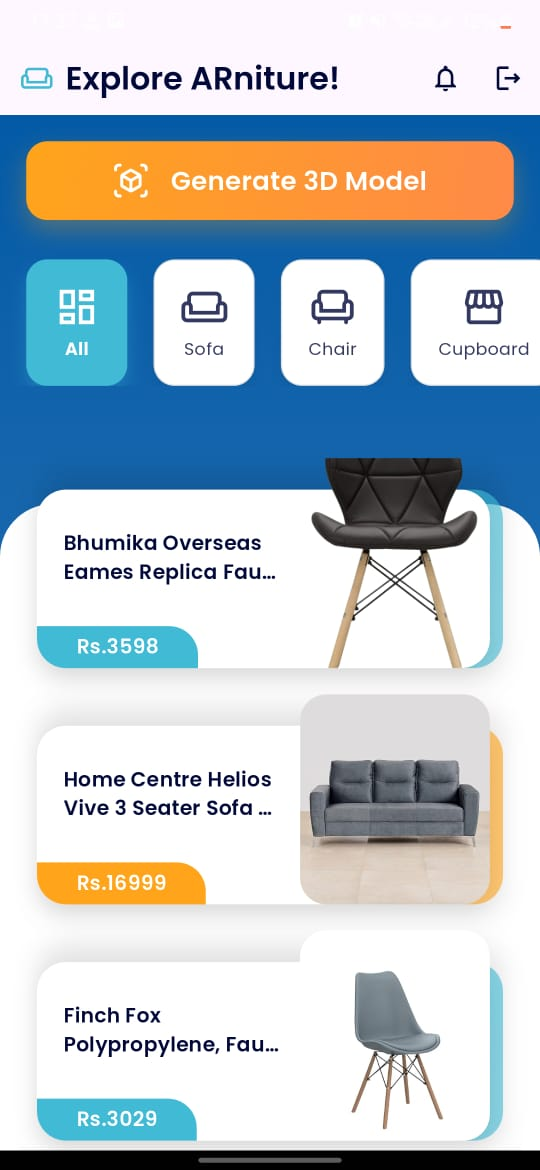
\includegraphics[width=0.75\linewidth]{fig_p4_1}
\caption{Figure 2}
\label{fig:2}
\end{figure}

Once authenticated, users are presented with a sample products screen (Figure 3) that displays a catalog of furniture items, organized by categories. This screen is critical for guiding the user experience by enabling easy navigation through available options. The interface is designed with clarity in mind, ensuring that users can effortlessly browse through different products and select items of interest.

\begin{figure}[htbp]
\centering
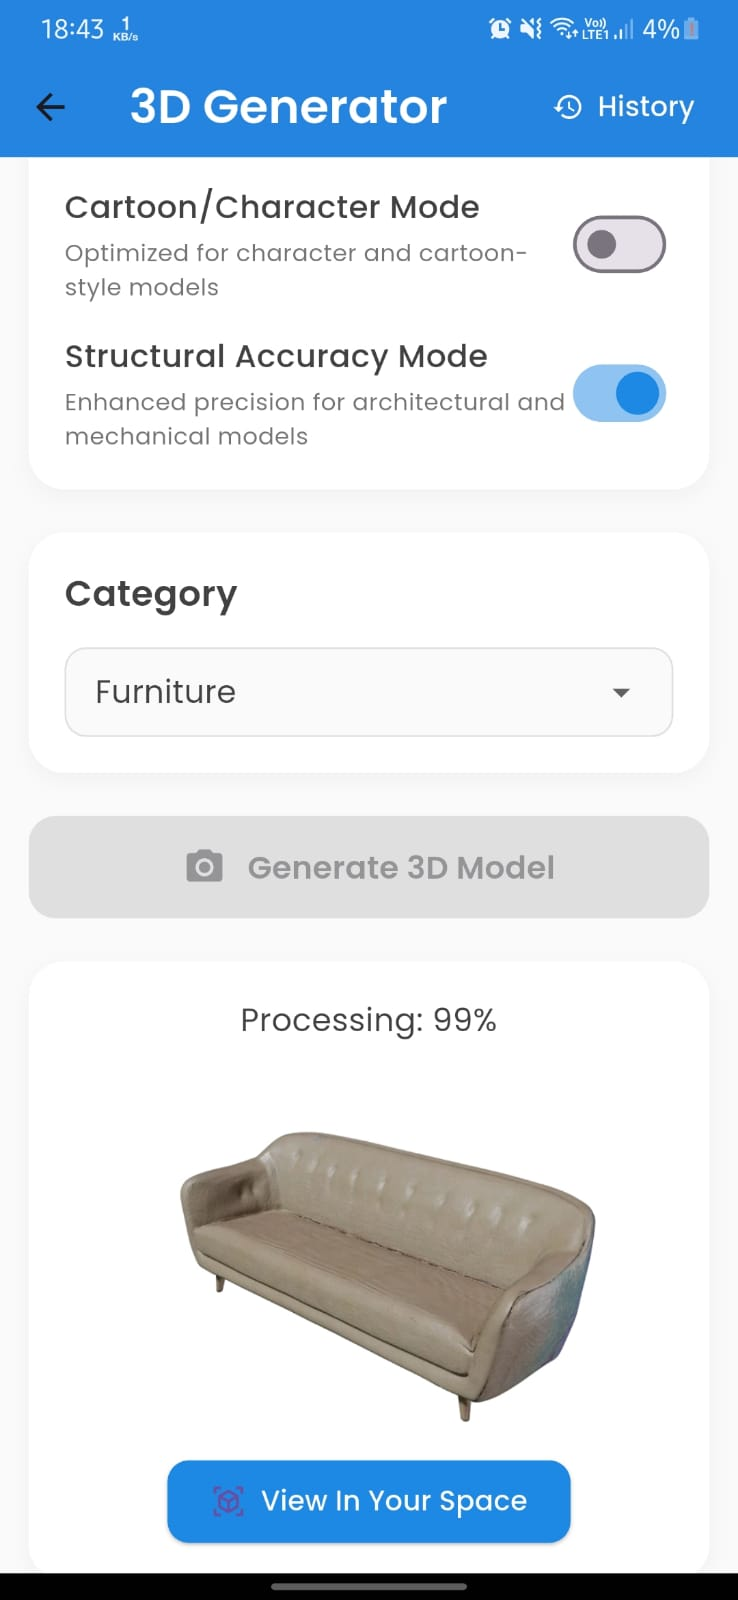
\includegraphics[width=0.75\linewidth]{fig_p4_2}
\caption{Figure 3}
\label{fig:3}
\end{figure}

When a user selects a product or opts to upload a new image, the system transitions to the 2D-to-3D model generation screen (Figure 4). Here, the application sends the image to the Meshy AI API, which processes it to generate a 3D model. Although this conversion process takes approximately 2--3 minutes, subsequent accesses to the same model are expedited by caching in Firebase Cloud Storage. This functionality is crucial for reducing redundant processing and enhancing the overall efficiency of the system.

\begin{figure}[htbp]
\centering

\includegraphics[width=0.75\linewidth]{fig_p4_0}
\caption{Figure 4}
\label{fig:4}
\end{figure}

Following model generation, the application presents the 3D model rendering screen (Figure 5). This module demonstrates how the system successfully converts a 2D image into a visually detailed 3D model, ready for interaction.

\begin{figure}[htbp]
\centering
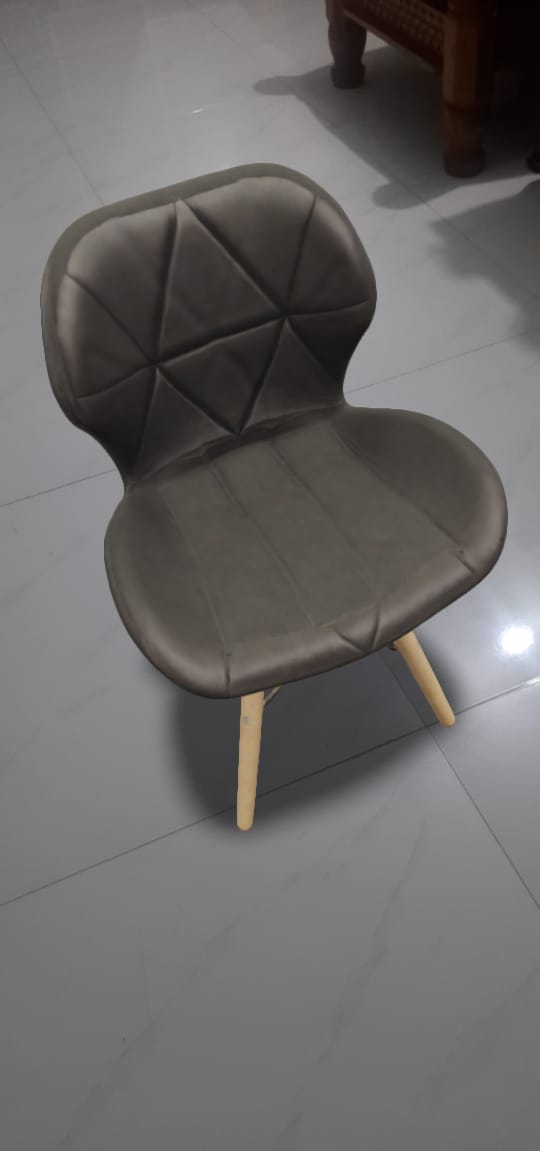
\includegraphics[width=0.75\linewidth]{fig_p5_2}
\caption{Figure 5}
\label{fig:5}
\end{figure}


\begin{figure}[htbp]
\centering
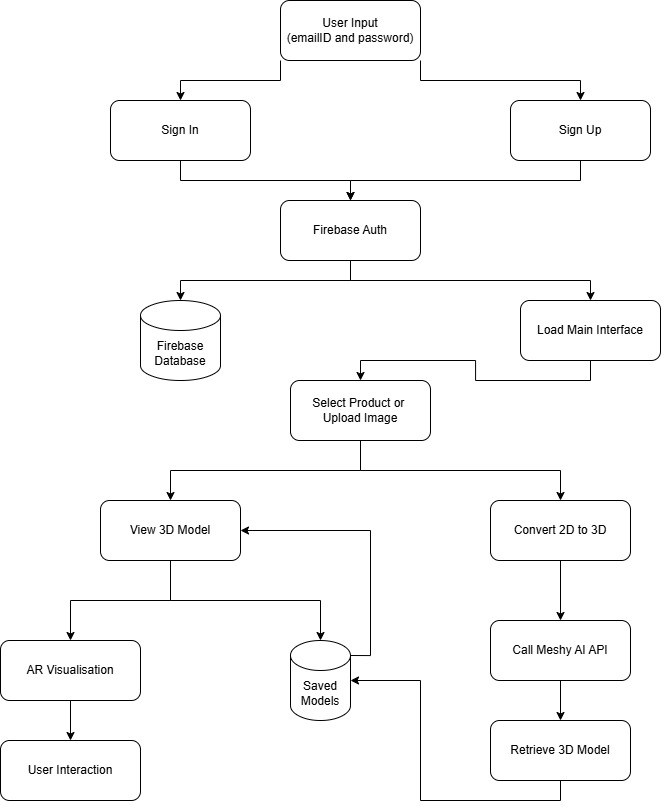
\includegraphics[width=0.75\linewidth]{fig_p3_0}
\caption{Figure 1}
\label{fig:1}
\end{figure}

\begin{figure}[htbp]
\centering
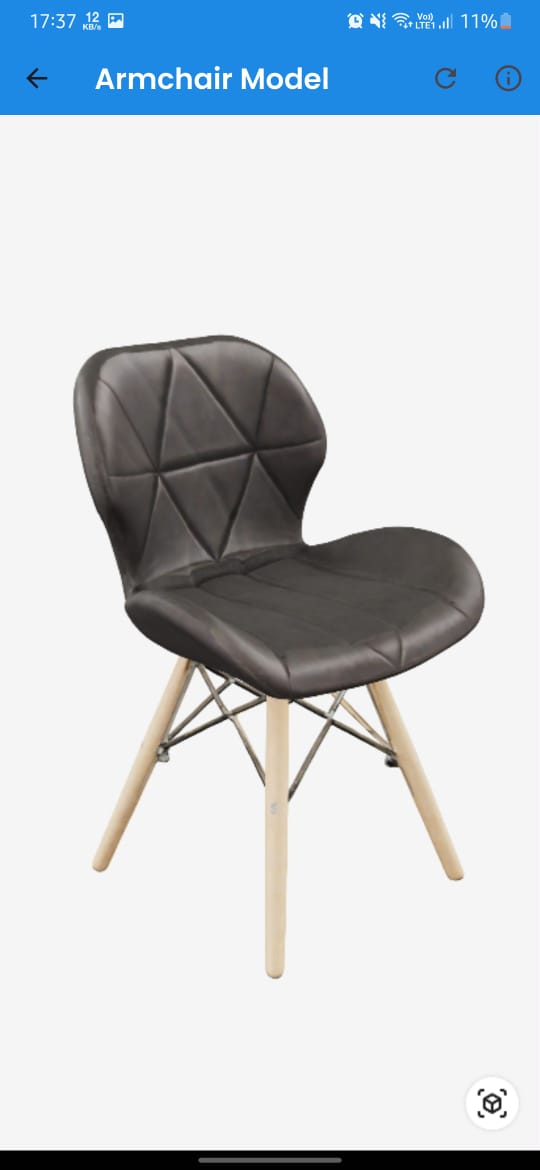
\includegraphics[width=0.75\linewidth]{fig_p5_0}
\caption{Figure 6}
\label{fig:6}
\end{figure}

\begin{figure}[htbp]
\centering
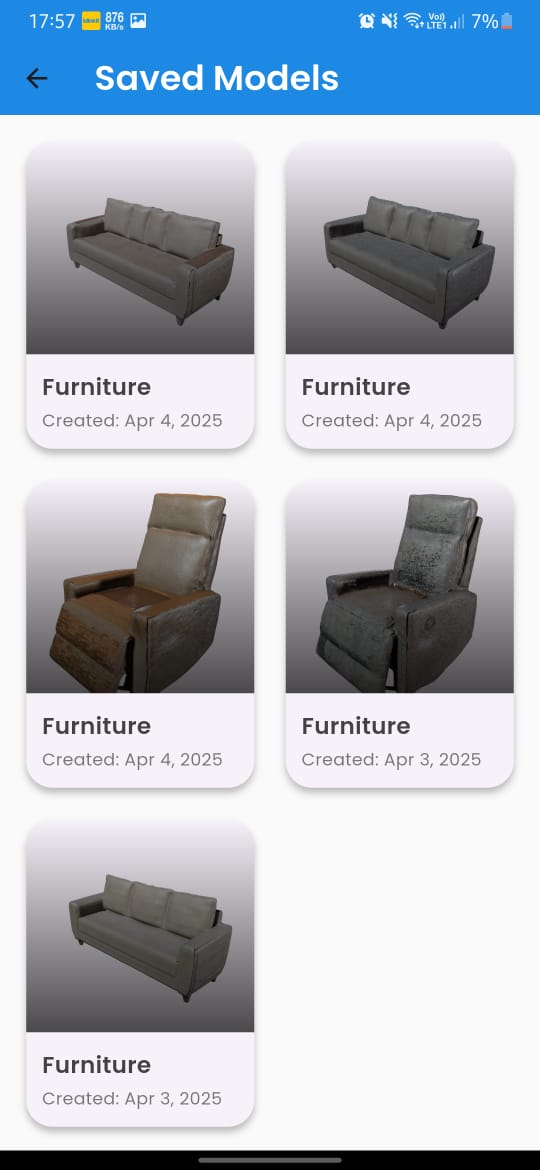
\includegraphics[width=0.75\linewidth]{fig_p5_1}
\caption{Figure 7}
\label{fig:7}
\end{figure}
\begin{thebibliography}{99}
\bibitem{ref1} [REF1]
\bibitem{ref2} [REF2]
\bibitem{ref3} [REF3]
\bibitem{ref4} [REF4]
\bibitem{ref5} [REF5]
\bibitem{ref9} [REF9]
\bibitem{ref10} [REF10]
\bibitem{ref17} [REF17]
\bibitem{ref19} [REF19]
\end{thebibliography}

\section{System Evaluation}
The quality of the system is evaluated based on visual fidelity and the accuracy of model details, ensuring that the output meets user expectations.

Figure 5 shows the 3D model rendering screen. Users can also view and interact with their previously generated models via the saved models (history) screen, as shown in Figure 6. This feature allows users to revisit and reuse models without reinitiating the conversion process, thereby optimizing system performance and enhancing the user experience by providing persistent access to their personalized catalog.

Figure 7 illustrates the AR functionality viewing screen. The core innovation of ARniture is realized in this module, which utilizes ARCore to overlay the 3D models in the user's real environment. The AR interface allows users to manipulate the model by rotating, scaling, and repositioning it, providing an immersive experience that is critical for informed decision-making in furniture selection. The application also adapts to different lighting conditions, ensuring that the model appears realistic in various environments. In summary, the experimental evaluation of ARniture indicates that the application effectively bridges the gap between digital visualization and real-world application. The system's integration of secure user authentication, dynamic 3D model generation, and real-time AR rendering demonstrates its potential to transform the online furniture shopping experience. While the 2D-to-3D conversion process poses a minor delay, caching strategies mitigate this drawback, and user feedback has been overwhelmingly positive. Future work will focus on optimizing the model generation pipeline and expanding interactive features to further enhance the overall experience.

\section{Future Work}
We want ARniture to move quickly for the users. Currently, it's too slow to turn a flat image into a 3D object. That doesn't excite people but also delays them. In future versions, we will see how to create 3D objects as quickly as possible so that the users will have immediate feedback. Our second goal is to introduce more objects through which people will be able to decorate their homes. So far, people have been able to put only furniture items within their bedrooms. We will introduce photographs on the wall, showpieces, and other home decoration pieces. We will also introduce some objects that simulate the characteristics of light in various rooms and provide users with the option of how materials appear. We would like more individuals to be able to utilize our app. Currently, ARniture will only be available on AR-compatible Android phones. We would like to make it so that we can utilize other devices in the future. This would include iPhones and computers. This way, individuals who have these other types of devices can use our program and design their space. Finally, we would also like to know from our users how ARniture can be further fine-tuned. We will have feedback channels where the users will be able to give feedback and understand how they are utilizing various features. We will track this information so that we understand what is working and what requires fine-tuning. We can then fine-tune accordingly so that we are actually improving our users' status.

\section{Conclusion}
This project presented ARniture, an augmented reality furniture online shopping experience enhancer. It has a Flutter frontend, rendering with ARCore, 2D image to 3D model conversion using Meshy AI API, and data storage with Firebase securely. ARniture allows users to easily and interactively visualize how the furniture can actually fit in their real space. The system was tested to verify that it closes the gap between viewing products on the internet and imagining them in actual situations and thus generating consumers' confidence in online shopping for furniture. Despite the fact that some of such issues, such as waiting for scanning 3D models, continue to exist, the system generally enhances the shopping experience. The app will also be optimized in the future further to transform models in less time and for more cross-platform apps, making ARniture as a scalable retail solution.

\begin{thebibliography}{99}
\bibitem{ref1} M. Azuma, "A Survey of Augmented Reality," Presence: Teleoperators and Virtual Environments, vol. 6, no. 4, pp. 355--385, 1997.
\bibitem{ref2} Google, "ARCore Overview," Google Developers, 2021. [Online]. Available: https://developers.google.com/ar
\bibitem{ref3} Google, "Flutter: Beautiful Native Apps in Record Time," Google Developers, 2021. [Online]. Available: https://flutter.dev
\bibitem{ref4} Firebase, "Firebase Documentation," Firebase, 2021. [Online]. Available: https://firebase.google.com/docs
\bibitem{ref5} Meshy AI, "Meshy AI API Documentation," Meshy AI, 2022. [Online]. Available: https://meshy.ai/docs
\bibitem{ref6} N. G. Tien, "Design and Development of an Augmented Reality Application for Furniture Retail," Journal of Emerging Technologies in Web Intelligence, vol. 12, no. 3, pp. 56--64, 2020.
\bibitem{ref7} S. Lee, "Mobile Augmented Reality for Retail," in Proc. IEEE Int. Symp. Mixed and Augmented Reality, 2019, pp. 50--57.
\bibitem{ref8} K. Kato, "User Experience Evaluation in AR Shopping Applications," Journal of Digital Retail, vol. 5, no. 2, pp. 89--96, 2018.
\bibitem{ref9} S. Smith, "Building Cross-Platform Apps with Flutter," Software: Practice and Experience, vol. 50, no. 3, pp. 250--255, 2020.
\bibitem{ref10} J. Brown, "Firebase: Real-Time Database for Mobile Applications," in Proc. Int. Conf. Cloud Computing, 2019, pp. 200--205.
\bibitem{ref11} A. Gupta, "Augmented Reality in E-Commerce: A Comparative Study," IEEE Trans. on Engineering Management, vol. 67, no. 2, pp. 215--223, 2020.
\bibitem{ref12} J. Martin, "Enhancing Furniture Visualization through Augmented Reality," in Proc. Global Conf. Consumer Electronics, 2021, pp. 300--305.
\bibitem{ref13} D. Lee, "Integrating AR with E-Commerce Platforms," Journal of Emerging Technologies, vol. 9, no. 1, pp. 130--137, 2021.
\bibitem{ref14} H. Park, "Mobile AR for Interior Design Applications," in Proc. Int. Conf. Mobile Services, 2019, pp. 78--83.
\bibitem{ref15} P. Hernandez, "AR and VR in Retail: Trends and Challenges," Journal of Retail Technology, vol. 3, no. 1, pp. 25--34, 2021.
\bibitem{ref16} T. Wong, "Augmented Reality: A New Dimension in Retail," IEEE MultiMedia, vol. 28, no. 2, pp. 45--52, 2021.
\bibitem{ref17} C. Davis, "Leveraging Flutter for Rapid Mobile App Development," IEEE Software, vol. 38, no. 4, pp. 50--55, 2021.
\bibitem{ref18} M. Patel, "Secure Mobile Applications using Firebase Authentication," in Proc. Int. Conf. Cybersecurity, 2020, pp. 140--145.
\bibitem{ref19} P. Kumar, "Modern Mobile Backend as a Service: A Case Study of Firebase," IEEE Cloud Computing, vol. 7, no. 2, pp. 20--27, 2020.
\bibitem{ref20} R. Singh, "Enhancing Mobile AR Applications with Cloud-Based Services," International Journal of Mobile Computing, vol. 10, no. 2, pp. 78--85, 2021.
\end{thebibliography}

\end{document}